\color{OffBlack}

{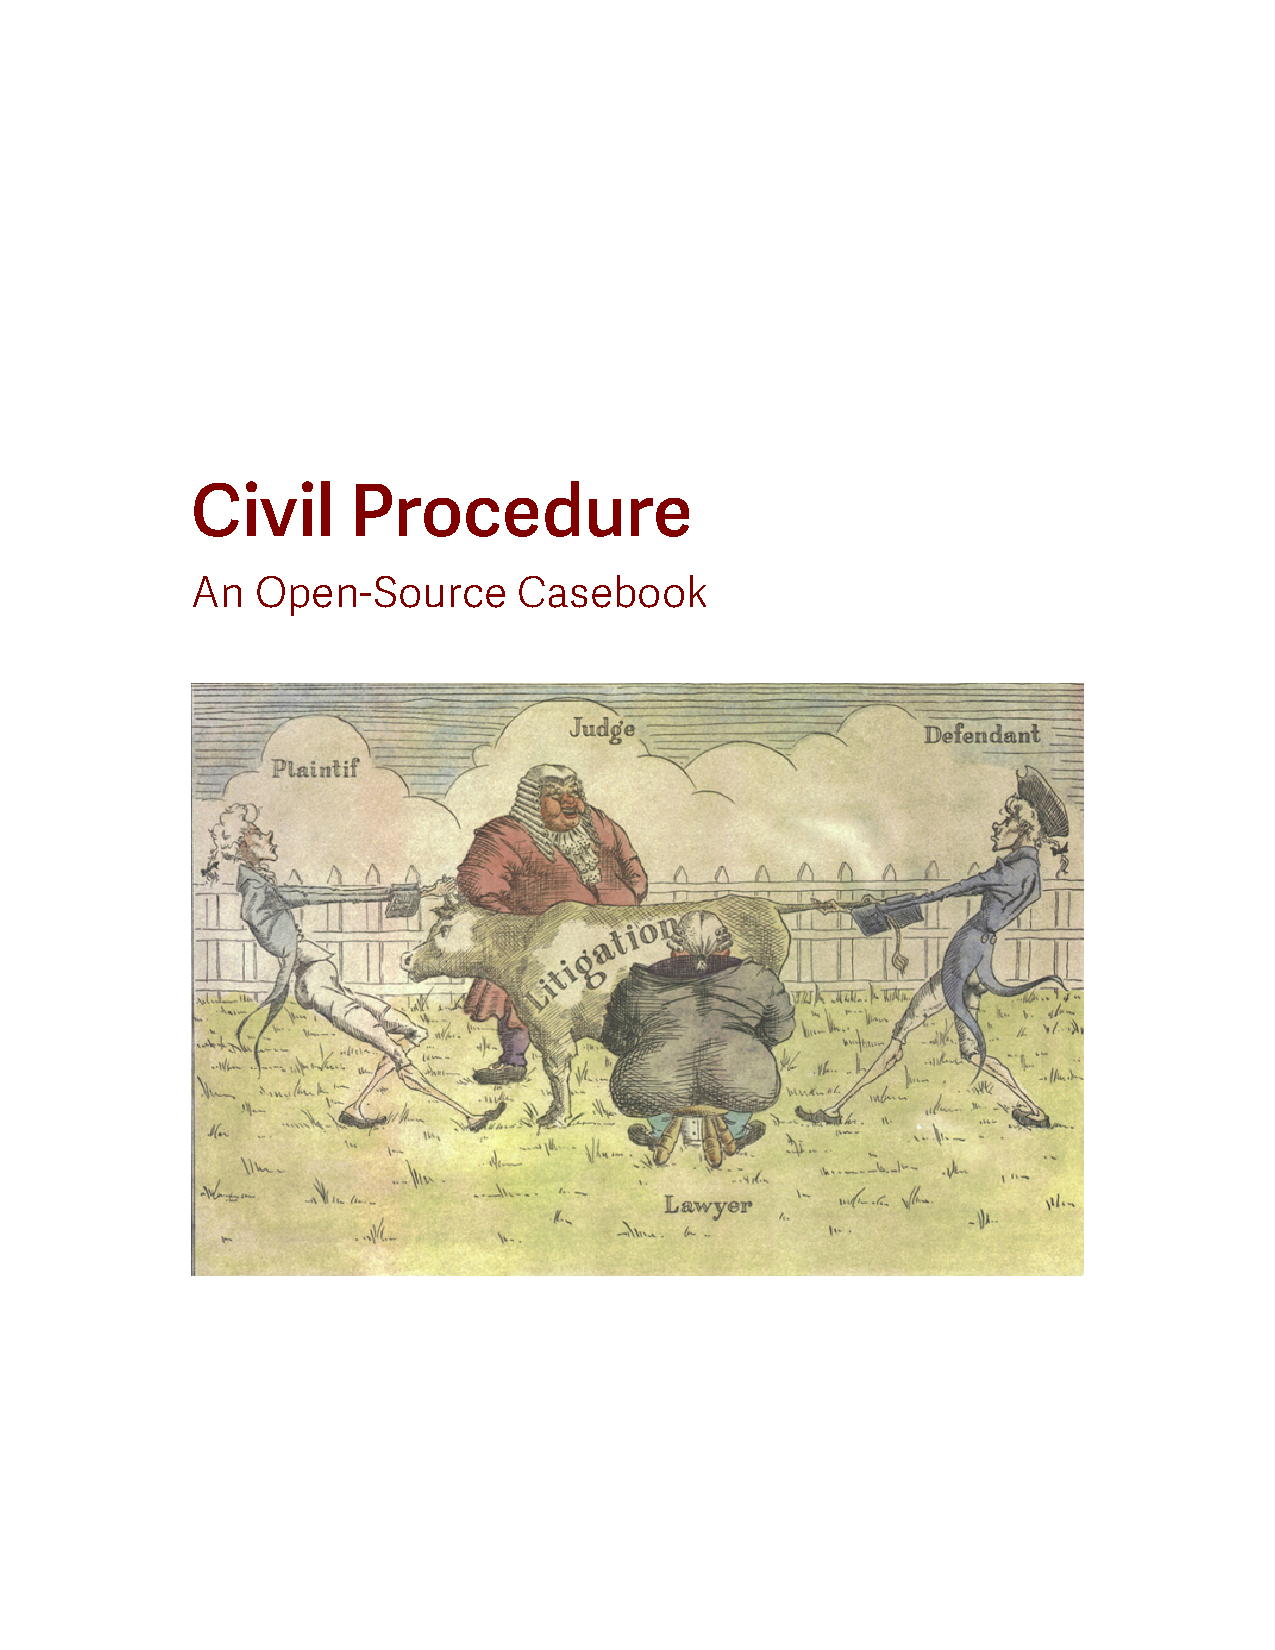
\includepdf{bookcover.pdf}\clearpage}{}

\blankpage

\blankpage

\blankpage

\frontmatter

\thispagestyle{empty}

\begin{flushright}

\vspace*{50mm}

{\bfseries\Huge{$title$}} 

{\bfseries\vspace{5mm}}

{\Large{An Open-Source Casebook}} 

\vspace{20mm}

{\normalsize{Eric M. Fink}} 

\vspace*{\fill}

\begin{small}

\rmfamily{Elon Law School}  

\rmfamily{\textit{Greensboro, North Carolina}}  

\rmfamily{\monthyear} 

\end{small}

\end{flushright}

\clearpage

\thispagestyle{empty}
\begingroup
\parindent 0pt
\vspace*{\fill}

\ccbyncsa

\begin{small}
\raggedright{This work is licensed under a Creative Commons Attribution-NonCommercial-ShareAlike 4.0 International License.} \\
\url{https://creativecommons.org/licenses/by-nc-sa/4.0/}

\vspace{1em}

Eric M. Fink\\
Associate Professor of Law \\
Elon University School of Law \\
Greensboro, North Carolina 27408 \\
\url{https://www.emfink.net/ElonLaw/}

\vspace{1em}

Source code: \url{https://github.com/EricMFink/$repo$}

\itshape{version $version$, \monthyear}

\end{small}
\endgroup

\clearpage

\thispagestyle{empty}

\topskip0pt
\vspace*{\fill}
\openepigraph{$epigraph$}{$epigraph-author$}{$epigraph-source$}
\vspace*{\fill}

\chapter*{Preface}

This book presents material for use in a first-year law school Civil Procedure course. Topics covered include the scope of a lawsuit (Party and Claim Joinder), selection of an appropriate forum (Personal and Subject Matter Jurisdiction), presentation of claims and defenses (Pleadings), choice of governing law (the {\textit{Erie}} doctrine), disposition without a trial (Summary Judgment), and the effect of judgments on future litigation (Claim and Issue Preclusion).

Most of the materials reproduced here are in the public domain; excerpts from copyrighted materials are included for teaching purposes under the fair use doctrine. Materials have been redacted to omit passages not pertinent to the learning objectives. Judicial opinions have also been "cleaned up" for ease of reading.\footnote{\textit{See} Jack Metzler, {\textit{Cleaning Up Quotations}}, 18 J. App. Prac. \& Process 143 (2017) (proposing "cleaned up" parenthetical for quotations from judicial opinions, to indicate the author “has removed extraneous, non-substantive material like brackets, quotation marks, ellipses, footnote reference numbers, and internal citations; may have changed capitalization without using brackets to indicate that change; and affirmatively represents that the alterations were made solely to enhance readability and that the quotation otherwise faithfully reproduces the quoted text.”)} 